\chapter{Results} \label{ch:conclusions}


Metrics were calculated using domain sizes ranging from 128x64 to 8192x4096 over 5000 frames. (In this case, a frame represents a complete time step wherein both E and H fields are updated.) For benchmarking purposes, the visualizer was disabled.

\begin{figure}[H]
	\centering
	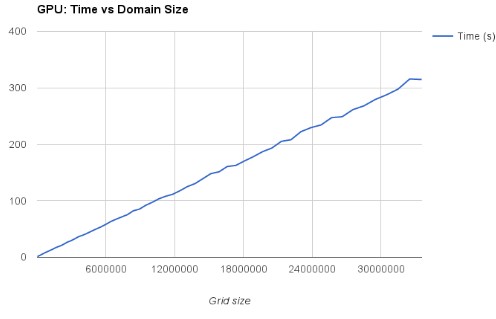
\includegraphics[width=\textwidth,
	keepaspectratio]{gpu_time_vs_domain_size.png}
	\caption{GoLightly: seconds for 5000 frames with the given domain size}
	\label{fig:gpuTimeVsDomainSize}
\end{figure}

As expected, As the number of computational cells in the simulation domain increases, the required computation time increases linearly.

\begin{figure}[H]
	\centering
	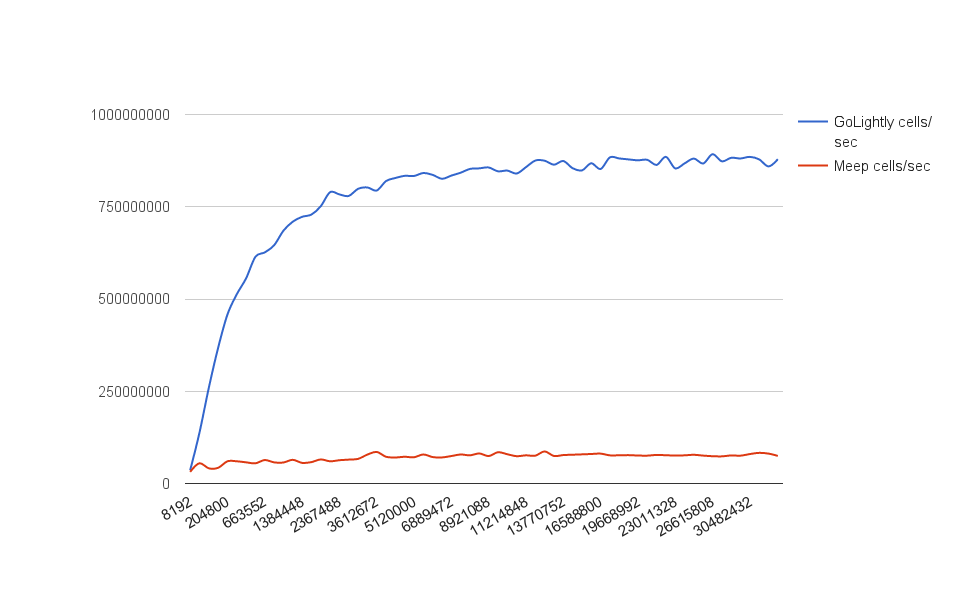
\includegraphics[width=\textwidth,
	keepaspectratio]{cells-per-second.png}
	\caption{GoLightly: Completed E and H updates per second}
	\label{fig:gridSizeVsComputeTime}
\end{figure}

Note that the total throughput (represented in the following figure as “cell” operations per second) increases dramatically as the domain size increases, until the point where GPU initialization overhead is outweighed by computation time.

Comparing to Meep:

\begin{figure}[H]
	\centering
	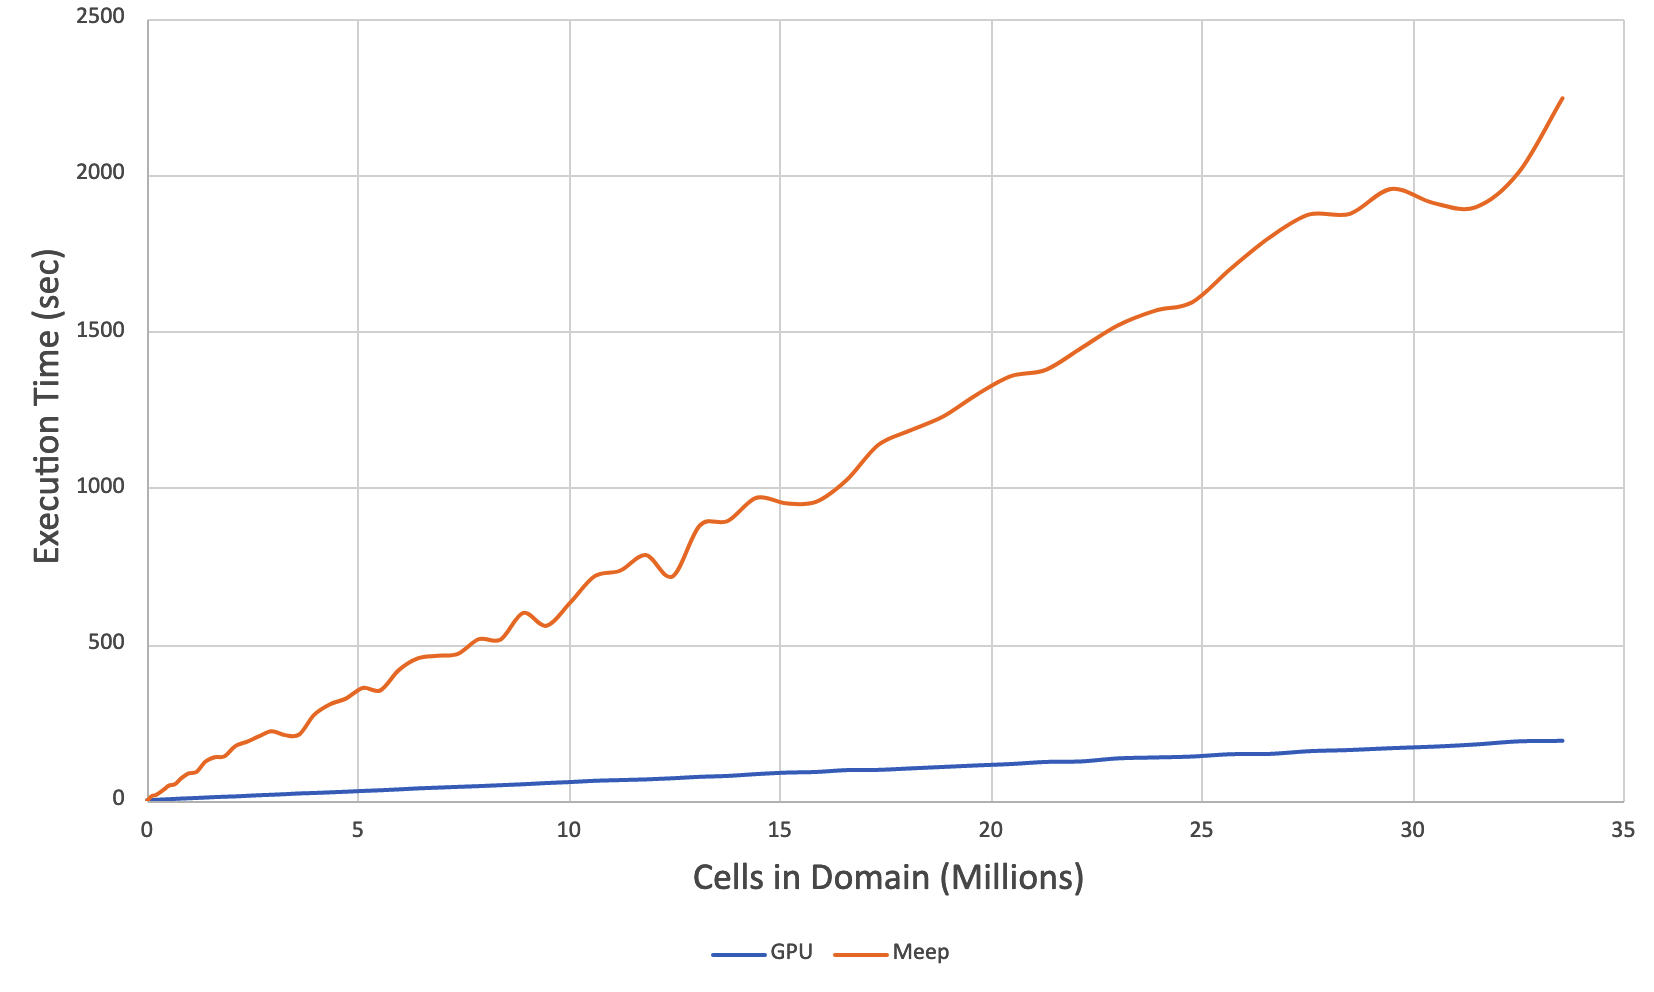
\includegraphics[width=\textwidth,
	keepaspectratio]{gpu-vs-meep.png}
	\caption{GoLightly vs Meep}
	\label{fig:gpuVsMeep}
\end{figure}

\begin{figure}[H]
	\centering
	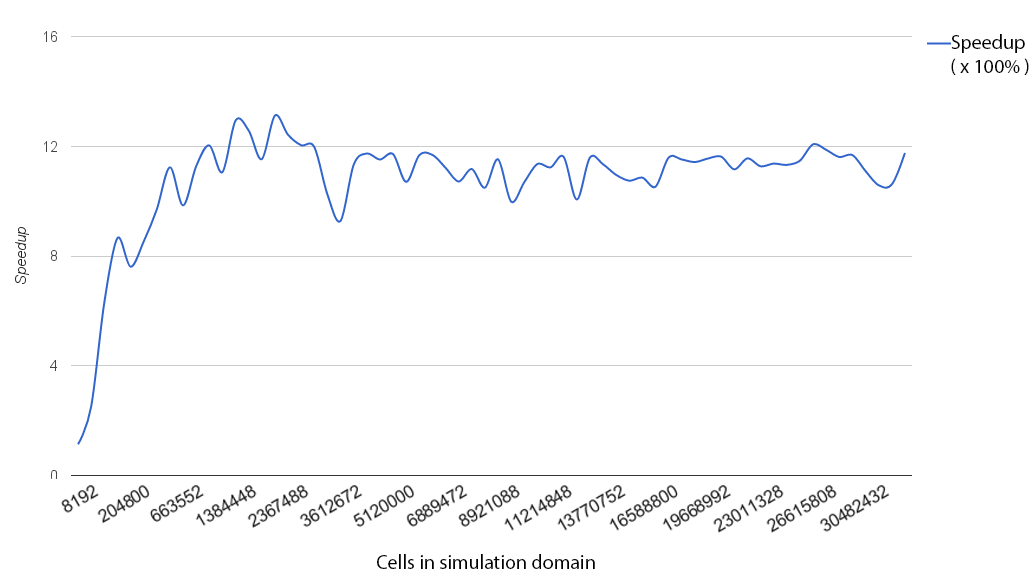
\includegraphics[width=\textwidth,
	keepaspectratio]{gpu-vs-meep-speedup.png}
	\caption{Speedup - Meep Time / GoLightly Time}
	\label{fig:gpuVsMeepSpeedup}
\end{figure}

This gives us a speedup ranging from 1.2 to 12, depending on the domain size. At lower resolutions, the overhead of initializing assets on the GPU can take more time than the simulation. In that case, a CPU-based simulation may outperform the GPU solution.

\section{Optimization and Enhancements}
Although a 1200\% speed increase is significant, there is much room for improvement. 





